%% LaTeX-Beamer template for KIT design
%% by Erik Burger, Christian Hammer
%% title picture by Klaus Krogmann
%%
%% version 2.1
%%
%% mostly compatible to KIT corporate design v2.0
%% http://intranet.kit.edu/gestaltungsrichtlinien.php
%%
%% Problems, bugs and comments to
%% burger@kit.edu

\documentclass[18pt]{beamer}

%% SLIDE FORMAT

% use 'beamerthemekit' for standard 4:3 ratio
% for widescreen slides (16:9), use 'beamerthemekitwide'

\usepackage{templates/beamerthemekit}
% \usepackage{templates/beamerthemekitwide}

%% TITLE PICTURE

% if a custom picture is to be used on the title page, copy it into the 'logos'
% directory, in the line below, replace 'mypicture' with the 
% filename (without extension) and uncomment the following line
% (picture proportions: 63 : 20 for standard, 169 : 40 for wide
% *.eps format if you use latex+dvips+ps2pdf, 
% *.jpg/*.png/*.pdf if you use pdflatex)

%\titleimage{mypicture}

%% TITLE LOGO

% for a custom logo on the front page, copy your file into the 'logos'
% directory, insert the filename in the line below and uncomment it

%\titlelogo{mylogo}

% (*.eps format if you use latex+dvips+ps2pdf,
% *.jpg/*.png/*.pdf if you use pdflatex)

%% TikZ INTEGRATION

% use these packages for PCM symbols and UML classes
% \usepackage{templates/tikzkit}
% \usepackage{templates/tikzuml}

% the presentation starts here

\title[Specification presentation]{Dynamic scheduler for scientific simulations}
\subtitle{Specification presentation}
\author{Kai Bittner, Ard Kastrati, Fabio Broghammer, Jan Ellmers, David Krenz, Benjamin-Philip Roth}

\institute{Steinbuch Centre for Computing (SCC)}

% Bibliography

\usepackage[citestyle=authoryear,bibstyle=numeric,hyperref,backend=biber]{biblatex}
\addbibresource{templates/example.bib}
\bibhang1em

\begin{document}

% change the following line to "ngerman" for German style date and logos
\selectlanguage{english}

%title page
\begin{frame}
\titlepage
\end{frame}

%table of contents
\begin{frame}{Outline}
\tableofcontents
\end{frame}

\section{Introduction}
	\begin{frame}{Introduction}
		\begin{itemize}
			\pause
			\item User-friendly middleware between scientific simulation and HPC
			\pause
			\item Runtime administration service for scientific simulations
			\pause
			\item Schedules large amount of individual tasks
			\pause
			\item Stores information in databases
			\pause
			\item Data mining of information
			\pause
			\item Dynamically changing of scheduling strategies
			\pause
			\item Bookkeeping for subsequent performance analysis
		\end{itemize}
	\end{frame}
	
\section{Features}
	\subsection{Required}
	\begin{frame}{Features (Required)}
		\begin{itemize}
			\pause
			\item Scheduling	
				\begin{itemize}
					\item Support of master worker and multi queue scheduling
					\item Support of different scheduling strategies
					\item Dynamic selection between provided scheduling strategies
				\end{itemize}
			\pause
			\item Usable with different scientific codes and task-types
			\pause
			\item Data mining
			\pause
			\item Bookkeeping
			\pause
			\item Visualization
		\end{itemize}
	\end{frame}
	
	\subsection{Optional}
	\begin{frame}{Features (Optional)}
		\begin{itemize}
			\pause
			\item Graphical user interface			
			\pause
			\item Dynamic change of MPI-World
		\end{itemize}
	\end{frame}
	
	\subsection{Demarcation}
	\begin{frame}{Features (Demarcation)}
		\begin{itemize}
			\pause
			\item Adaptive learning
		\end{itemize}
	\end{frame}

\section{Scenario}
	\begin{frame}{Scenario (1)}
		Scenario to show connection between functional requirements:
		\pause
		\begin{itemize}
			\item Start the dynamic scheduler via moab:
			\item 'msub run\_scheduler.sh'
		\end{itemize}
		\begin{block}{run\_scheduler.sh}
			\#MSUB -l nodes=2:ppn=6 \\
			\#MSUB -l walltime=0:10:00 \\
			\#MSUB -l pmem=200mb \\
			\#MSUB -q multinode \\
			mpirun \textbf{scheduler -design master-worker}
		\end{block}
	\end{frame}
	\begin{frame}{Scenario (2)}
		\center -activity diagram in image viewer-
	\end{frame}

\section{Self-imposed conditions}
	\begin{frame}{Self-imposed conditions}
		\begin{tabular}{|c|c|c|c|c|}\hline
			& very important & important & less important & unimportant\\ \hline
			Robustness & x &&&\\ \hline
			Reliability & x &&&\\ \hline
			Correctness & x &&&\\ \hline
			Usability &&& x &\\ \hline
			Efficiency & x &&&\\ \hline
			Portability &&& x &\\ \hline
			Compatibility &&& x &\\ \hline
			Modifiability & x &&&\\ \hline
			Security &&& x &\\ \hline
			
		\end{tabular}
	\end{frame}
	
\section{Visualization}
	\begin{frame}{Visualization}
		\begin{itemize}
			\pause
			\item 1. Plot: Task interconnection tree
			\pause
			\item 2. Plot: Task-flow diagram
			\pause
			\item 3. Plot: Usage-time diagram
		\end{itemize}
	\end{frame}
	
	\begin{frame}{Task interconnection tree}
		\begin{center}
			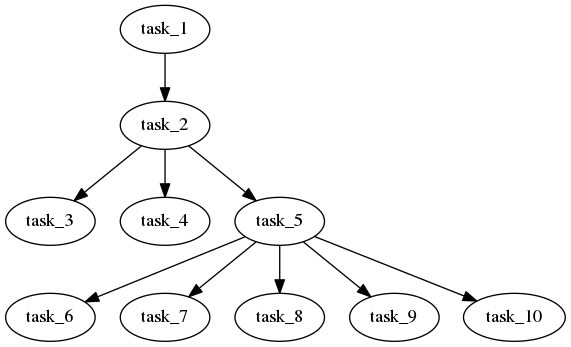
\includegraphics[width=220px, height=150px]{images/task.png}
		\end{center}
	\end{frame}
	
	\begin{frame}{Task-flow diagram}
		\begin{center}
			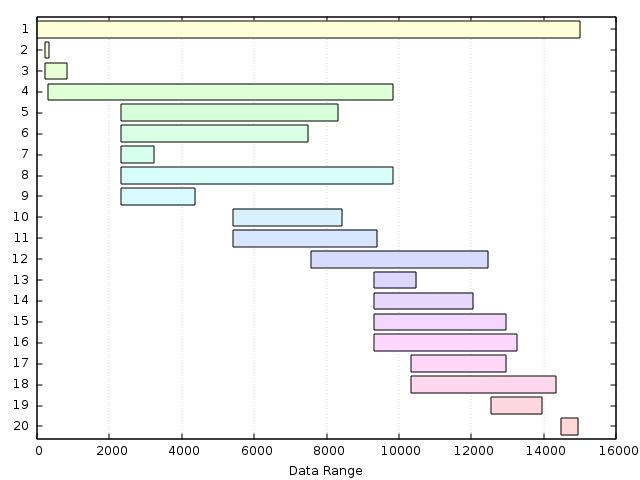
\includegraphics[width=280px, height=190px]{images/taskflow.png}
		\end{center}		
	\end{frame}
	
	\begin{frame}{Usage-time diagram}
		\begin{center}
			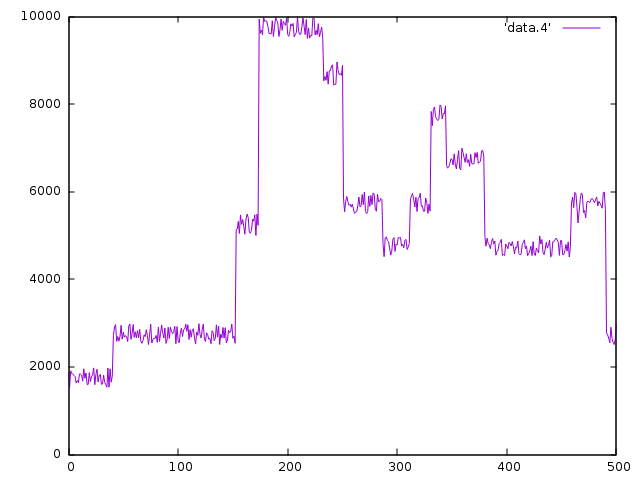
\includegraphics[width=280px, height=190px]{images/nodeusage.png}
		\end{center}		
	\end{frame}
	
	\begin{frame}
		\begin{center}
			The END
		\end{center}		
	\end{frame}
	
\end{document}
